\documentclass[a4paper]{article} 
\addtolength{\hoffset}{-2.25cm}
\addtolength{\textwidth}{4.5cm}
\addtolength{\voffset}{-3.25cm}
\addtolength{\textheight}{5cm}
\setlength{\parskip}{0pt}
\setlength{\parindent}{0in}

\usepackage[square,sort,comma,numbers]{natbib}
\usepackage{blindtext} % Package to generate dummy text
\usepackage{charter} % Use the Charter font
\usepackage[utf8]{inputenc} % Use UTF-8 encoding
\usepackage{microtype} % Slightly tweak font spacing for aesthetics
\usepackage{amsthm, amsmath, amssymb} % Mathematical typesetting
\usepackage{float} % Improved interface for floating objects
\usepackage{hyperref} % For hyperlinks in the PDF
\usepackage{graphicx, multicol} % Enhanced support for graphics
\usepackage{xcolor} % Driver-independent color extensions
\usepackage{pseudocode} % Environment for specifying algorithms in a natural way
\usepackage[mmddyy]{datetime} % Uses YEAR-MONTH-DAY format for dates

\usepackage{fancyhdr} % Headers and footers
\pagestyle{fancy} % All pages have headers and footers
\fancyhead{}\renewcommand{\headrulewidth}{0pt} % Blank out the default header
\fancyfoot[L]{} % Custom footer text
\fancyfoot[C]{} % Custom footer text
\fancyfoot[R]{\thepage} % Custom footer text
\newcommand{\note}[1]{\marginpar{\scriptsize \textcolor{red}{#1}}} % Enables comments in red on margin

\DeclareMathOperator*{\argmin}{arg\,min}

%----------------------------------------------------------------------------------------


%-------------------------------
%	TITLE VARIABLES (identify your work!)
%-------------------------------

\newcommand{\yourname}{Balthazar Neveu | Jamy Lafenetre}
\newcommand{\youremail}{balthazarneveu@gmail.com | jamy.lafenetre@ens-paris-saclay.fr}
\newcommand{\assignmentnumber}{4}

\begin{document}

%-------------------------------
%	TITLE SECTION (do not modify unless you really need to)
%-------------------------------
\fancyhead[C]{}
\hrule \medskip
\begin{minipage}{0.295\textwidth} 
\raggedright
\footnotesize
\yourname \hfill\\
\youremail
\end{minipage}
\begin{minipage}{0.4\textwidth} 
\centering 
\large 
Lab session \# \assignmentnumber\\ 
\normalsize 
NPM 2024\\ 
\end{minipage}
\begin{minipage}{0.295\textwidth} 
\raggedleft
\today\hfill\\
\end{minipage}
\medskip\hrule 
\bigskip




%-------------------------------
%	ASSIGNMENT CONTENT (add your responses)
%-------------------------------


\section*{Question 1}
The octree depth is the parameter that has the most impact on the result, but also on the
computation time. We highlight this impact in figure \ref{fig:SPR_octree}.
Bigger values lead to a deeper tree and more scale for the SPR solving.
It can also increase drastically the number of voxels present on the finest scale, which can
lead the linear system solving to become non-tractable.
If the number of scales is too low (we show the result for $n=6$), the voxel grid is too
coarse to represent the geometry and we can therefore notice blocky artifacts.
If the number of scales is too high ($n=10$), then the grid may become too fine for the sample
density. The implicit discretization of integrals done in the Galerkin solver no longer
holds, as there are too few samples within each voxel. This results in high-frequency artifacts.

\begin{figure}[ht]
    \centering
    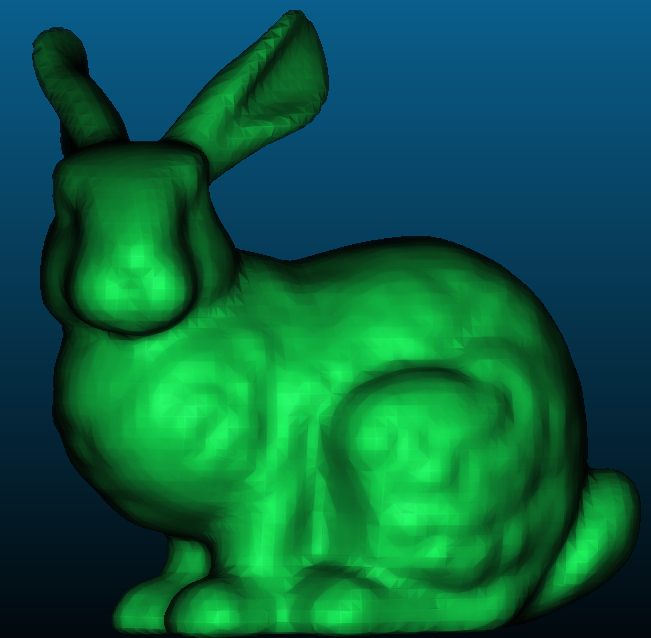
\includegraphics[width=0.3\linewidth]{figures/n=06.png}
    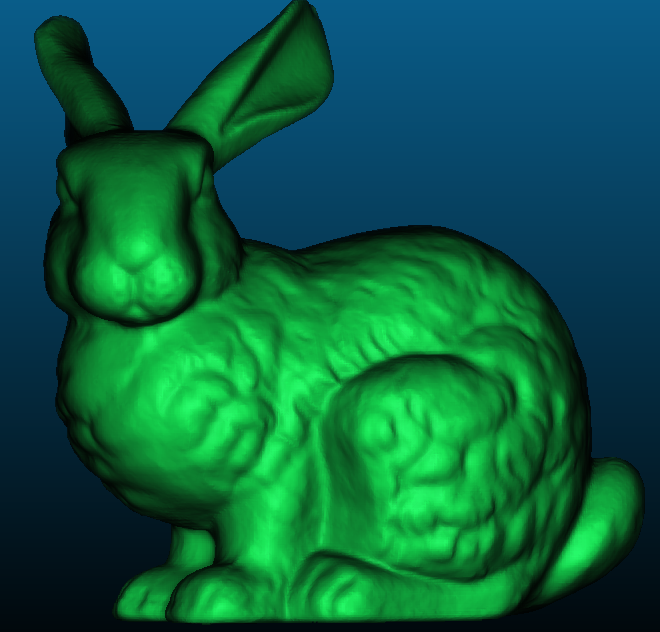
\includegraphics[width=0.3\linewidth]{figures/n=08 .png}
    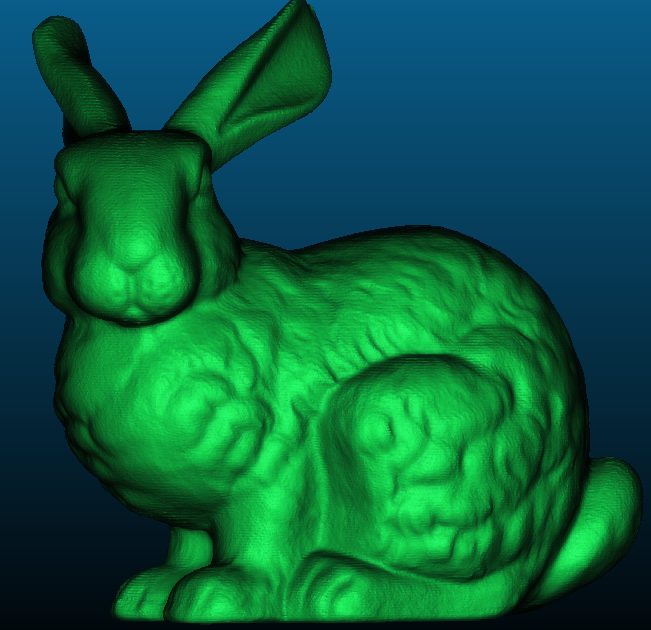
\includegraphics[width=0.3\linewidth]{figures/n=10.png}
    \caption{From left to right: screened Poisson reconstruction with 6, 8, and 10 scales.}
    \label{fig:SPR_octree}
\end{figure}

We can also tweak the number of samples per node to ensure that each node has enough samples.
The built-in plugin claims that higher values such as 15 are preferable for noisy clouds.
This is indeed plausible, as the low-frequency Bezier kernel used in the solver will integrate
many samples within a single voxel to attenuate noise.
For clouds without noise, using such high values will prevent the voxel hierarchy from
populating the finest level, therefore resulting in some local blocky artifacts.
Additional artifacts can be visible around structures featuring very high frequencies,
because the leaf voxels are too coarse for the local geometry. This can be seen in figure \ref{fig:SPR_spn}.

\begin{figure}[ht]
    \centering
    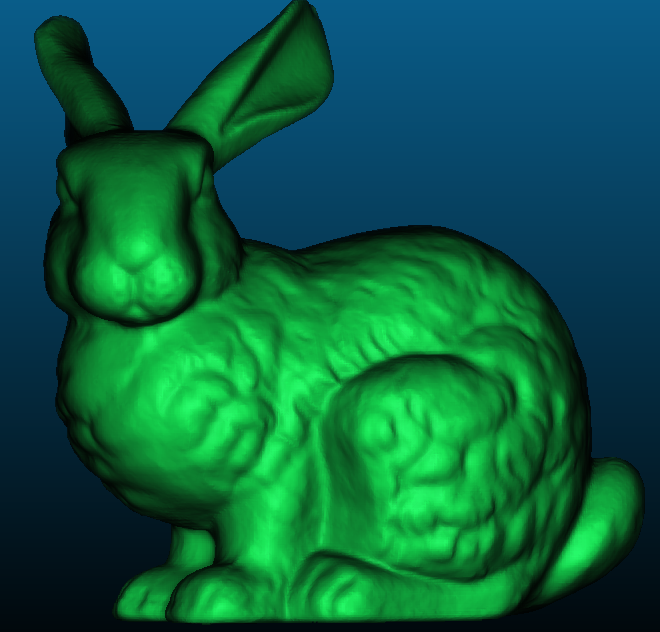
\includegraphics[width=0.3\linewidth]{figures/n=08 .png}
    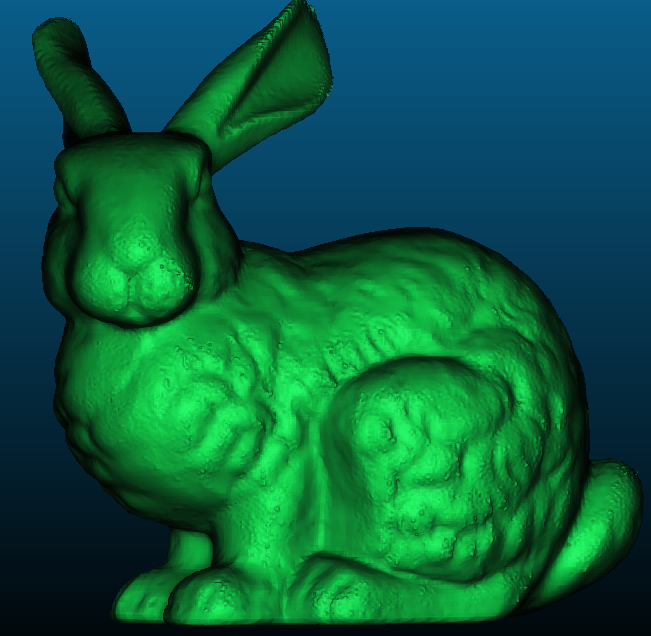
\includegraphics[width=0.3\linewidth]{figures/n=08_15_spn.png}
    \caption{From left to right: screened Poisson reconstruction on 8 scales, for 1.5 and 15 maximum samples per node.}
    \label{fig:SPR_spn}
\end{figure}

The regularization weight (dubbed "point weight" in CloudCompare) drives the screening
importance of the SPR. Lower values give a smooth surface, whereas very high values will
"overfit" the cloud and the noise. We compare different values in figure \ref{fig:SPR_pw}.
\begin{figure}[ht]
    \centering
    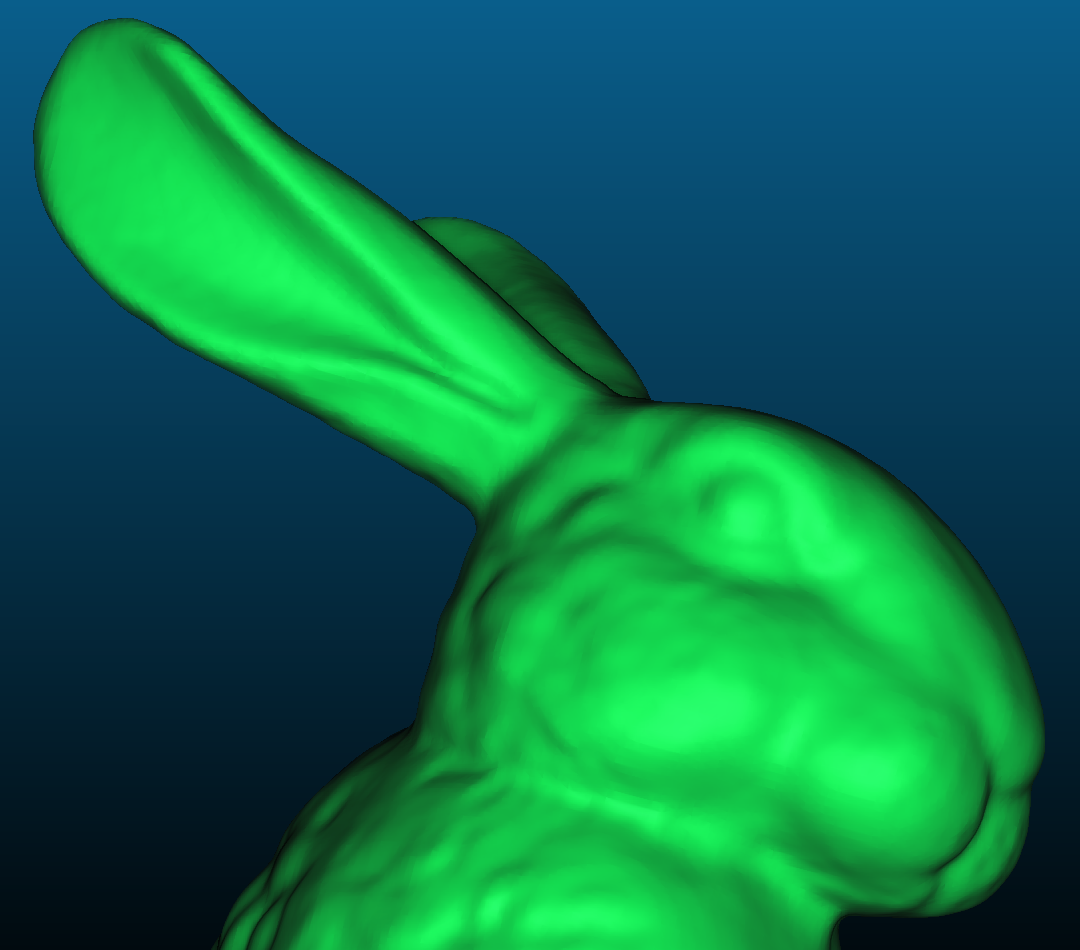
\includegraphics[width=0.3\linewidth]{figures/n=08_00_pw.png}
    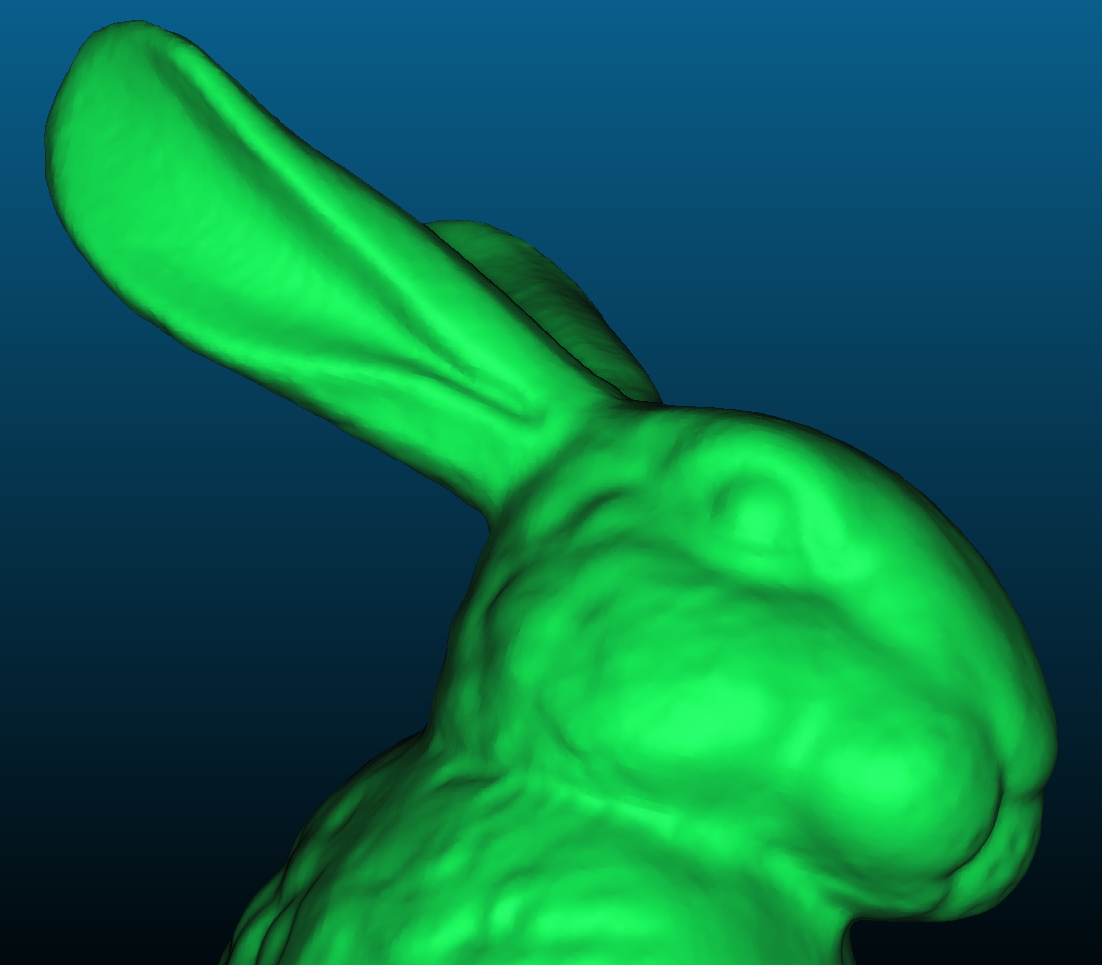
\includegraphics[width=0.3\linewidth]{figures/n=08_2_pw.png}
        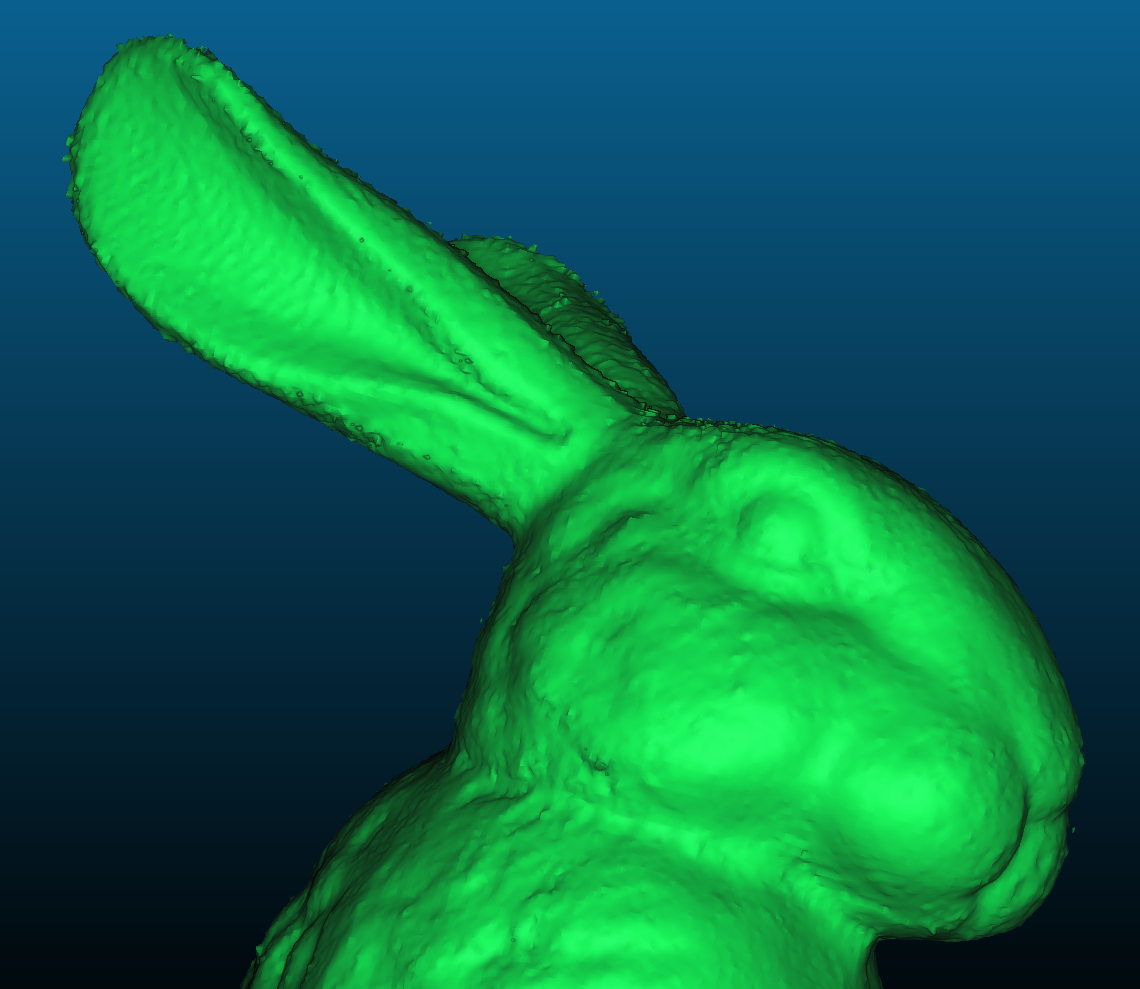
\includegraphics[width=0.3\linewidth]{figures/n=08_20_pw.png}
    \caption{From left to right: screened Poisson reconstruction on 8 scales, for a point weight of 0, 2, and 20.}
    \label{fig:SPR_pw}
\end{figure}


The given point cloud has very little noise, and the bunny is a very smooth closed structure.
With a maximum tree depth of 8, a maximum sample-per-node value of 1.5, and a point weight value
of 2, we were able to obtain the most satisfactory reconstruction. In our case, a satisfactory
reconstruction is a mesh that preserves the global smoothness of the bunny, without losing
the few sharper details and without displaying grid artifacts or spiky artifacts.

The resulting mesh is composed of 373,800 triangles.

\section*{Questions 2-3}
We compare our handcrafted Hoppe implementation with the SPR plugin of CloudCompare.
Qualitative results can be seen in figure \ref{fig:hoppe_vs_spr}, and the quantitative results are 
reported in table \ref{tab:HoppeTable}. Our implementation takes 22 seconds to run
on the bunny cloud, which is mostly due to the single-threaded kd-tree implementation we use.
If we neglect the interaction with the tree and do the processing on a GPU,
our reconstruction takes around 17ms. A better optimization could realistically lower this
overhead to a few milliseconds.
SPR takes between 1 and 2 seconds to compute a surface.

\begin{figure}[ht]
  \centering
  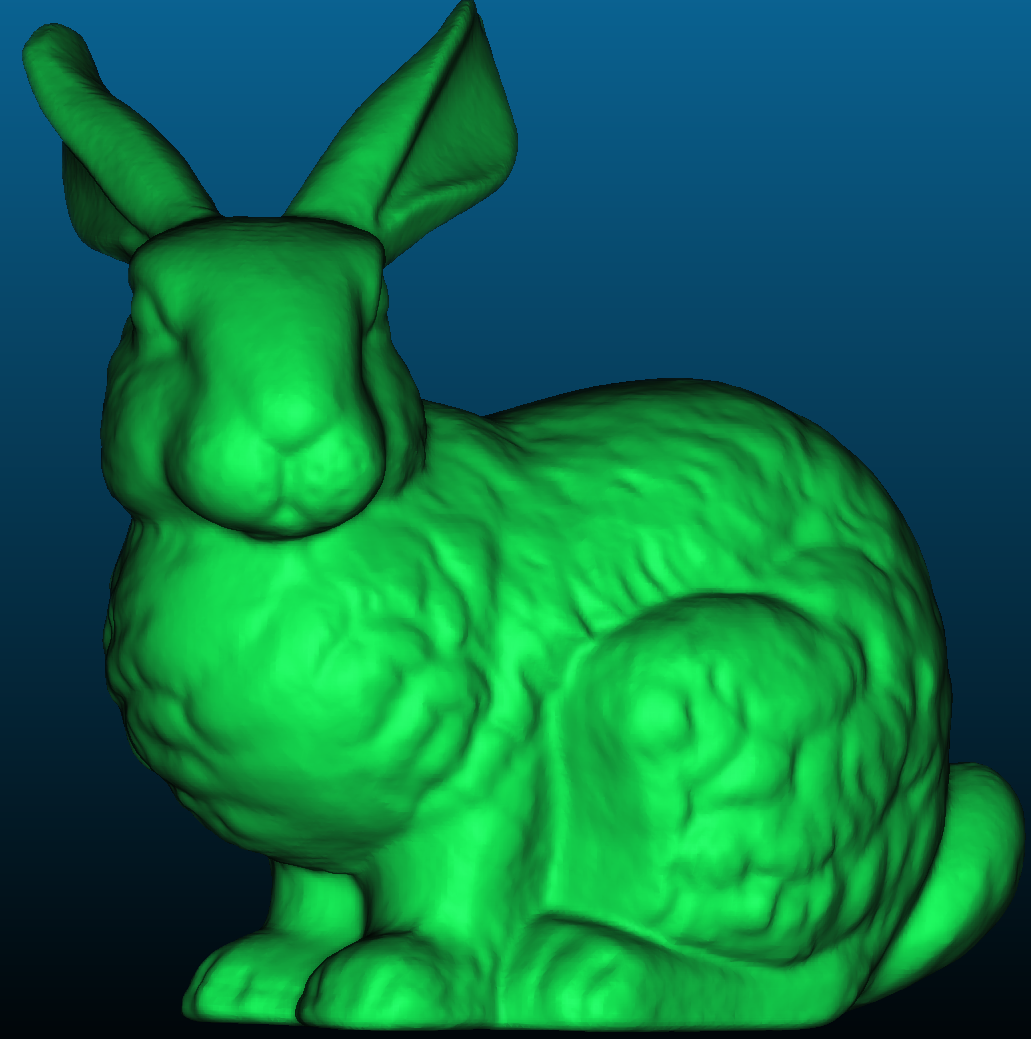
\includegraphics[width=0.3\linewidth]{figures/SPR.png}
  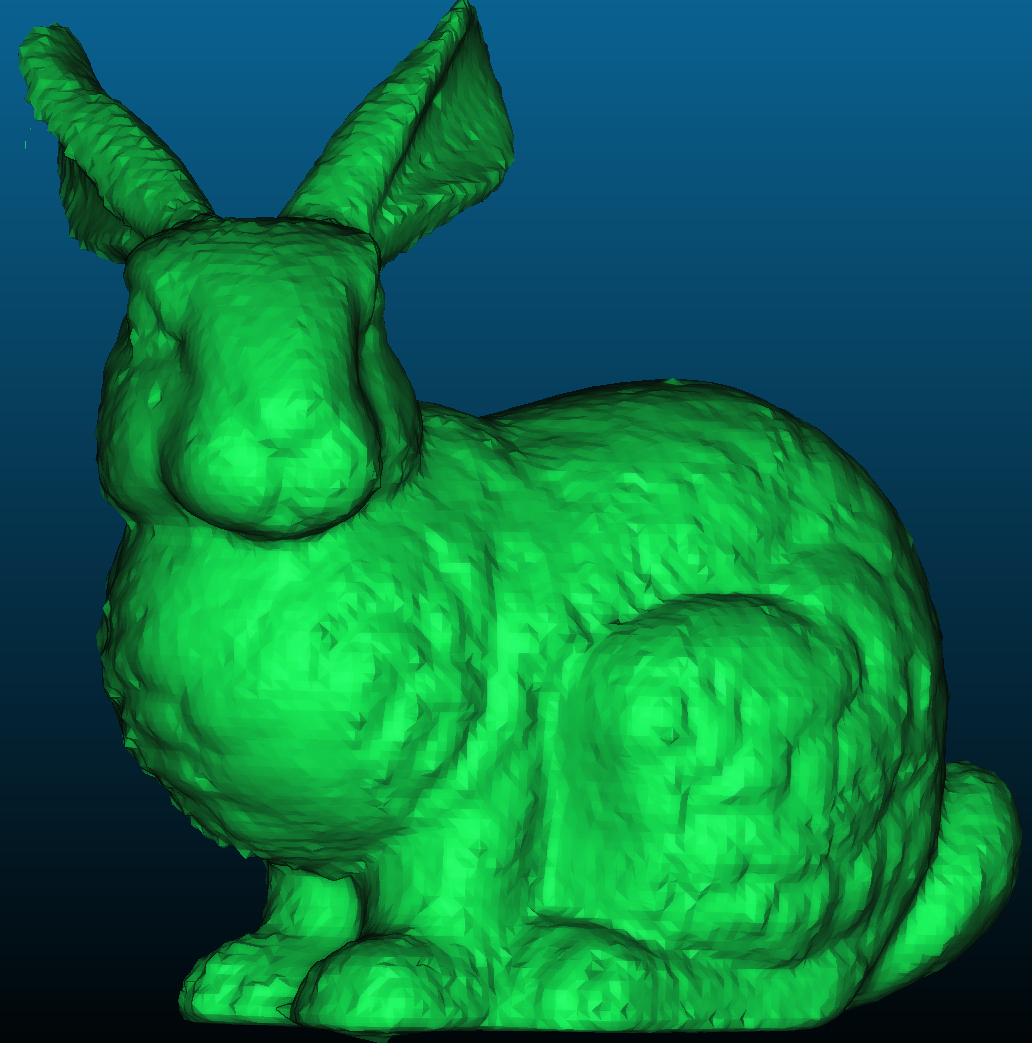
\includegraphics[width=0.3\linewidth]{figures/Hoppe.png}
  \caption{Left: SPR reconstruction. Right: our Hoppe reconstruction.}
  \label{fig:hoppe_vs_spr}
\end{figure}

\begin{table}
    \centering
    \begin{tabular}{|c|c|c|}
      \hline
         & SPR & Hoppe \\
      \hline
      Computation time & ~ 1s & ~10ms \\
      Number of triangles & 32 168 & 373 800 \\
      Quality of reconstruction & High & Poor \\
      \hline
    \end{tabular}
    \caption{Comparison between our Hoppe implementation and SPR.}
    \label{tab:HoppeTable}
  \end{table}

\section*{Question 4}
We run the same comparison as before with our handcrafted implementation of IMLS,
and compare the result in figure \ref{fig:hoppe_vs_imls_vs_spr} and table \ref{tab:IMLSTable}. We use
the same strategy as before to approximate the execution time. The result is
smoother and more satisfactory than with Hoppe, at the cost of a few
more operations. We can observe that IMLS is able to recover smooth structures such
as the ears of the bunny accurately, contrary to Hoppe. However, only SPR can recover small details
such as the nose.

\begin{figure}[ht]
  \centering
  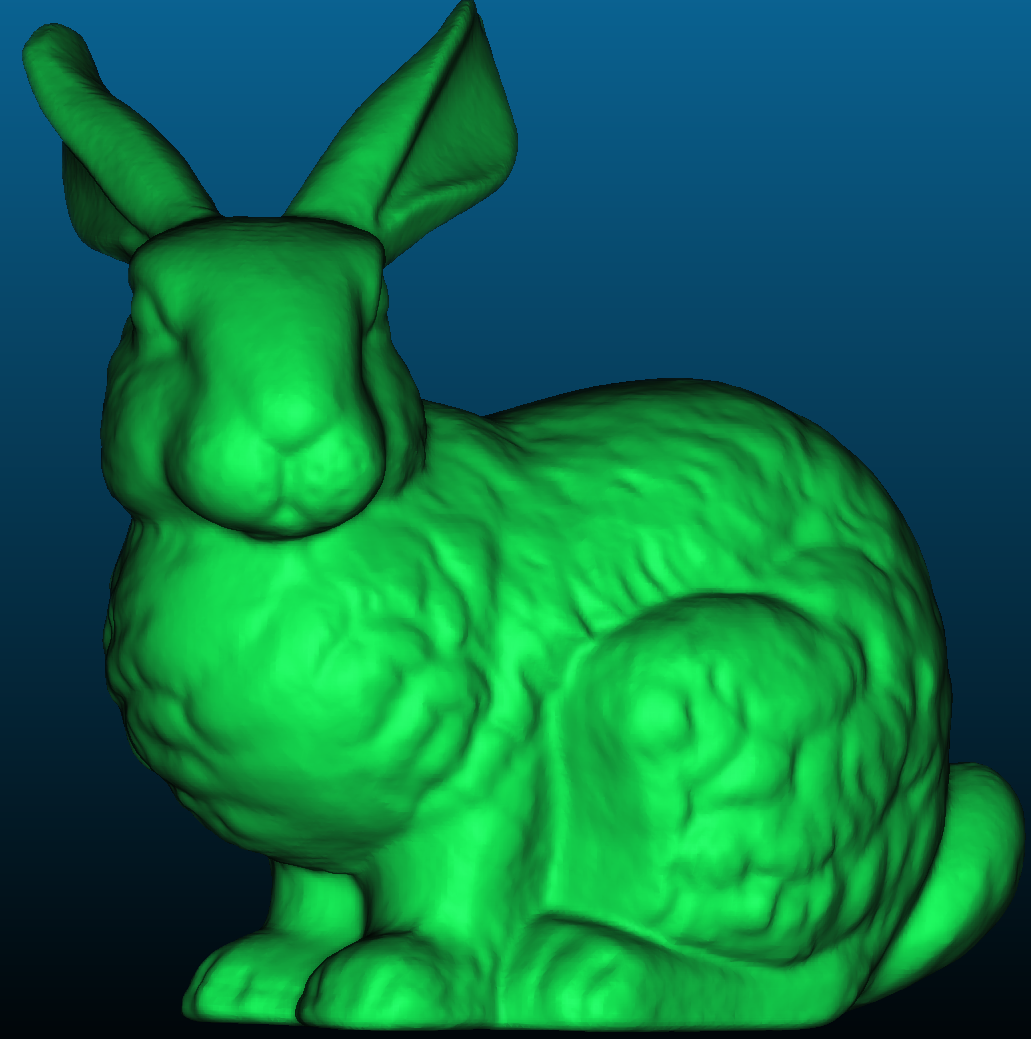
\includegraphics[width=0.3\linewidth]{figures/SPR.png}
  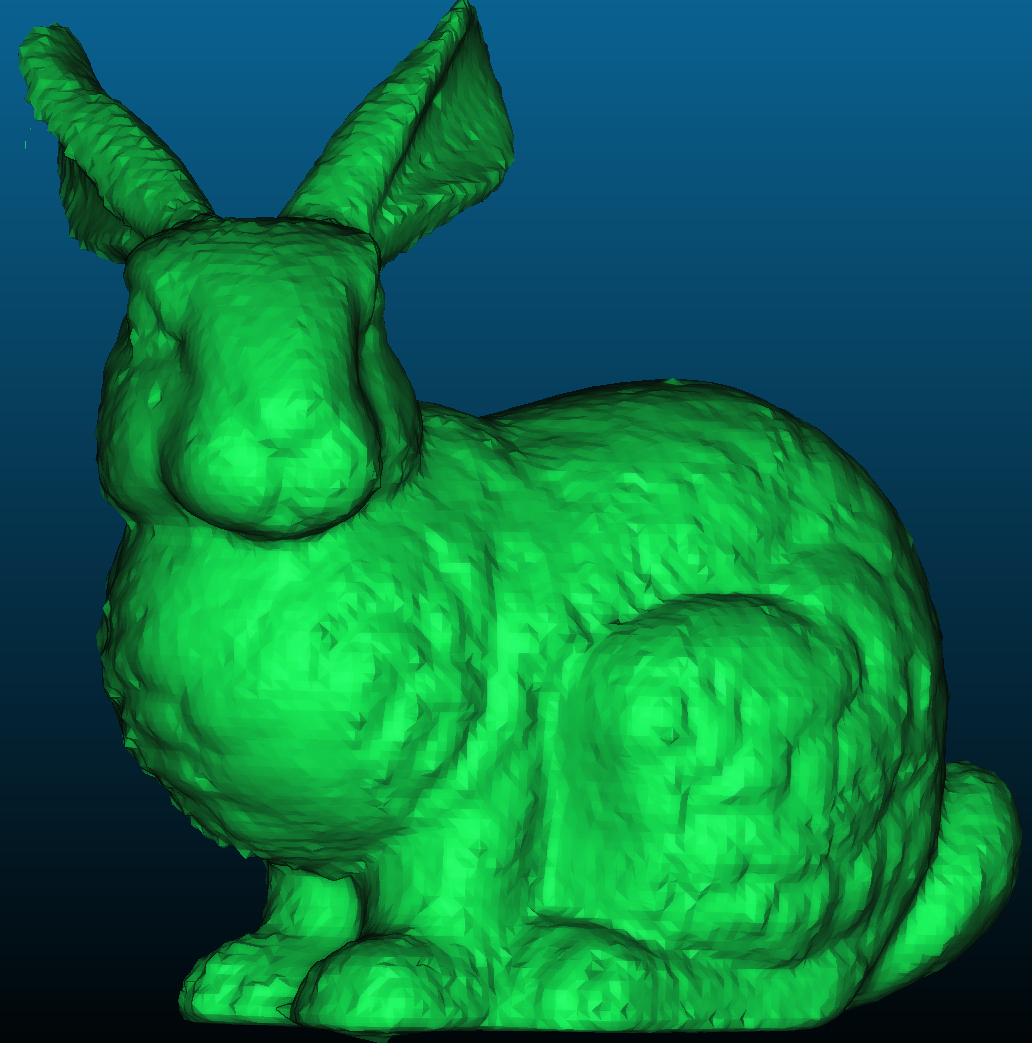
\includegraphics[width=0.3\linewidth]{figures/Hoppe.png}
  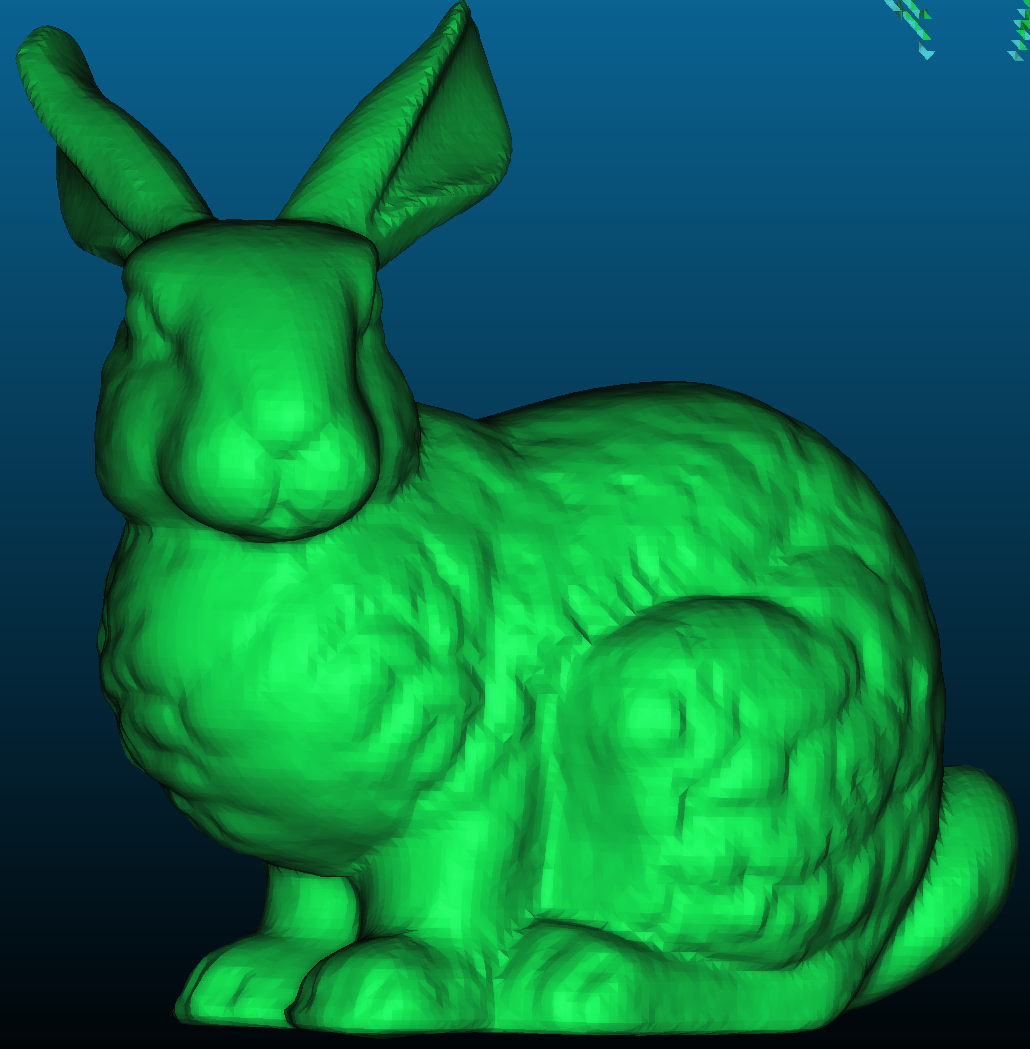
\includegraphics[width=0.3\linewidth]{figures/IMLS.png}
  \caption{Left: SPR reconstruction. Middle: our Hoppe reconstruction. Right: our IMLS reconstruction.}
  \label{fig:hoppe_vs_imls_vs_spr}
\end{figure}

\begin{table}
    \centering
    \begin{tabular}{|c|c|c|c|}
      \hline
         & SPR & Hoppe & IMLS\\
      \hline
      Computation time & ~ 1s & ~ 10ms & ~ 100ms\\
      Number of triangles & 373 800 & 32 168 & 77 164\\
      Quality of reconstruction & High & Poor & Medium\\
      \hline
    \end{tabular}
    \caption{Comparison between our implementation of Hoppe, IMLS and SPR.}
    \label{tab:IMLSTable}
  \end{table}


\end{document}

